\chapter{Le maillage}\label{Ch-mesh}
\begin{abstract}
À ce niveau du document, on peut considérer que la méthode des éléments finis a été présentée, au moins en ce qui concerne les aspects les plus classiques (et même un peu plus).
Nous avons décidé, avant d'entrer dans le détail de «subtilités» liées au comportement des matériaux et à la non-stationnarité, d'insérer ici un petit chapitre sur le maillage, dont les techniques de construction n'ont rien de commun avec celles relatives aux éléments eux-mêmes.
De plus, nous nous restreindrons aux maillages de type Delaunay.\index[aut]{Delaunay (Boris Nikolaïevitch), 1890-1980, Russe}-Voronoï\index[aut]{Voronoï (Gueorgui Feodossievitch), 1868-1908, Russe}
\end{abstract}

Le maillage n'a pas seulement un intérêt en calcul scientifique. Le maillage est un «support» de représentation tridimensionnel utilisé par exemple dans les jeux vidéo ainsi que dans les animations 3D. Dans ce dernier cas, on s'intéresse à la qualité du maillage en lien avec la qualité de rendu de l'image générée lorsque l'on applique une texture sur le maillage. On s'intéresse également à comment «faire bouger» le maillage pour qu'un personnage n'apparaissent pas distordu pendant une animation...

\medskip
L'opération de maillage peut se faire à partir de plusieurs données:
\begin{itemize}
   \item soit à partir de données à utiliser pour la discrétisation: sommets, arêtes...
   \item soit à partir de données de type CAO décrivant uniquement les entités géométriques.
\end{itemize}
Nous nous contenterons de présenter quelques outils de maillage relatifs au premier cas, i.e. lorsque nous disposons de points, arêtes... mais le second cas n'est pas vraiment plus compliqué.


\medskip
%\section{Stratégies de maillage}
%
Les \textcolorblue{méthodes de construction de maillage} sont essentiellement:
\begin{itemize}
   \item Maillage par triangles/tétraèdres:
   \begin{itemize}
      \item Méthodes utilisant le critère de Delaunay:\index[aut]{Delaunay (Boris Nikolaïevitch), 1890-1980, Russe} les bases de la méthode seront exposées au paragraphe~\ref{Sec-MeshDelau};
      \item Méthodes par avancement de fronts: le principe en sera détaillé au paragraphe~\ref{Sec-MeshFront};
      \item Méthodes par décomposition spatiale;
   \end{itemize}
   \item Maillage par quadrangles/hexaèdres: quelques remarques seront faites au paragraphe~\ref{Sec-MeshQuad}
   \begin{itemize}
      \item Maillage par avancement de fronts;
      \item Maillage par décomposition en domaines.
   \end{itemize}
\end{itemize}

\medskip
Parfois, il ne s'agit pas de mailler un domaine, mais de le remailler.
Les \textcolorblue{méthodes d'adaptation de maillage} les plus connues sont:
\begin{itemize}
   \item Raffinement;
   \item Transformation des éléments;
   \item Déplacements de nœuds;
   \item Simplification de maillage.
\end{itemize}

L'utilisation de différentes méthodes est illustré à la figure~\ref{Fig-MeshAlliez} issue de~\cite{bib-Alliez}.
\begin{figure}[htb]
\begin{center}
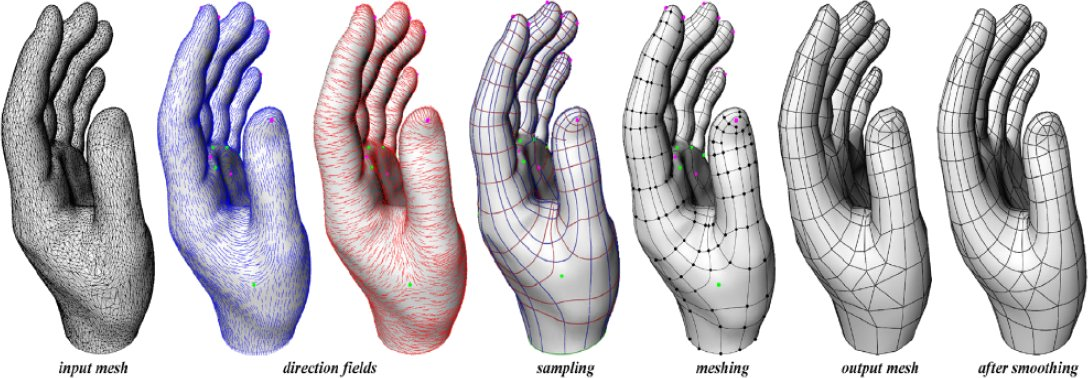
\includegraphics[height=50mm]{M-transfo.jpg}
\end{center}
\caption{Manipulations sur des maillages}\label{Fig-MeshAlliez}
\end{figure}

\medskip
\section{Maillage de Delaunay}\label{Sec-MeshDelau}

\medskip
\subsection{Maillage simplexial}

L'opération de maillage consiste à discrétiser un domaine (i.e. un milieu continu ou plutôt sa modélisation géométrique) par des éléments 
(éléments finis nous concernant), si possible bien proportionnés: 
au paragraphe \ref{Sec-mesh-carac}, nous avons déjà présenté les dimensions géométriques représentatives d'un maillage que sont 
le diamètre maximum des éléments $h$\index{élément fini!diamètre d'un} et le facteur de forme du maillage\index{facteur de forme du maillage} 
$\sigma$, ainsi que le diamètre $h_K$ d'un élément $K$\index{élément fini!diamètre d'un} et sa rondeur $\rho_K$\index{élément fini!rondeur d'un}.
Ces deux derniers paramètres sont représentés sur la figure \ref{h-rho}. 

\medskip
Dans ce chapitre, nous traiterons du cas bidimensionnel.
Nous expliquerons les bases théoriques, mais ne rentrerons pas dans les détails pratiques de la programmation
d'algorithmes de maillage (il y a de très bons cours disponibles sur le sujet).

\medskip
Dans la suite nous aurons besoin des notions suivantes:
\begin{itemize}
   \item un \textcolorblue{segment fermé} (resp. ouvert) d'extrémités $a$ et $b$ de $\RR^d$ est noté $[a,b]$ (resp. $]a,b[$);
   \item un \textcolorblue{convexe} $E$ est un ensemble tel que: $\forall \intervalle{a}{b}\in E^2, [a,b]\subset E$;
   \item le \textcolorblue{convexifié} d'un ensemble $E$ de points de $\RR^d$, noté $\mathcal{C}(E)$ est le plus petit convexe
	contenent $E$.
   \item un domaine $\Omega$ (i.e. un ouvert de $\RR^d$) est dit \textcolorblue{polygonal} si son bord $\Gamma=\partial\Omega$
	est formé d'un nombre fini de segments;
   \item un \textcolorblue{n-simplex $(x_0, ..., x_n)$} est le convexifié des $n+1$ points de $\RR^d$ affine indépendant.
	Cela implique que $n\le d$. Les sommets sont des 0-simplex, un segment est un 1-simplex, un triangle un 2-simplex, un tétraèdre est un 3-simplex.
\end{itemize}


\medskip
\begin{definition}[Maillage simplexial]
Un maillage simplexial~$\mathcal{T}_{d,h}$ d'un ouvert polygonal~$\Omega_h$ de~$\RR^d$ est un ensemble de~$d$-simplex~$K^k$ de~$\RR^d$ pour~~$k = 1... N_t$, tel que l'intersection de deux~$d$-simplex distincts~$\overline{K}^i$ et~$\overline{K}^j$ de~$\mathcal{T}_{d,h}$ soit l'ensemble vide ou le $p$-simplex commun à~$\overline{K}^i$ et~$\overline{K}^j$ avec~$p\le d$.

En termes plus simples: le maillage~$\mathcal{T}_{d,h}$ est constitué de~$N_t$ éléments~$K^k$ ($k = 1... N_t$) appelés~$d$-simplex (qui sont des triangles pour~$d=2$ et des tétraèdres pour~$d=3$) tels que l'intersection (de l'adhérence) de deux éléments~$\overline{K}^i$ et~$\overline{K}^j$ soit soit nulles (éléments parfaitement séparés), soit un  point, une arête ou une face (i.e. un~$p$-simplex avec~$p\le d$) commun aux deux éléments.
\end{definition}

On notera~$\mathcal{T}_{0,h}$ l'ensemble des sommets de~$\mathcal{T}_{d,h}$, $\mathcal{T}_{1,h}$ l'ensemble de ses arêtes et~$\mathcal{T}_{d-1,h}$ l'ensemble de ses faces.
Le bord $\partial\mathcal{T}_{d,h}$ est l'ensemble des faces n'appartenant qu'à un seul~$d$-simplex de~$\mathcal{T}_{d,h}$

\begin{theoreme}
Pour tout ouvert polygonal $\Omega_h$ de $\RR^2$, il existe un maillage de cet ouvert sans sommet interne (voir figure~\ref{Fig-Mext}).
\end{theoreme}
Les sommets de ce maillage sont les points anguleux du bord $\partial\Omega_h$.

Malheureusement ce théorème n'est plus vrai en dimension plus grande que 2, car il existe des configurations d'ouvert polyédrique non-convexe qu'il est impossible de mailler sans point interne.
\begin{figure}[htb]
\begin{center}
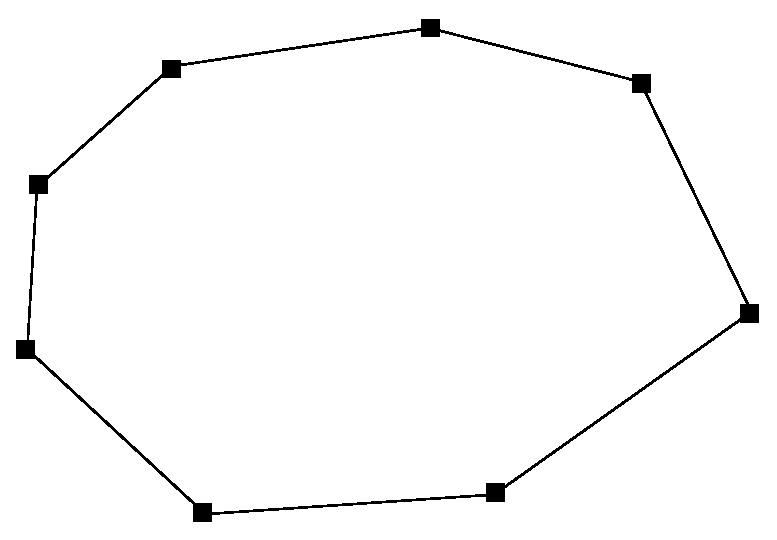
\includegraphics[height=25mm]{ext1.eps} \hspace{2em} 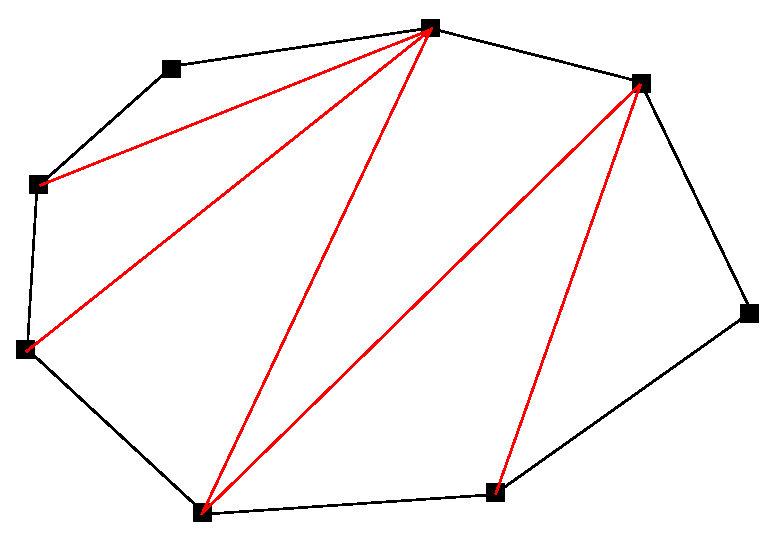
\includegraphics[height=25mm]{ext2.eps}
\end{center}
\caption{a) Points et arêtes et b) maillage de Delaunay sans point interne}\label{Fig-Mext}
\end{figure}


\medskip
\subsection{Maillage de Delaunay-Voronoï}\index{maillage de Delaunay-Voronoï}

Dans le cas général, la construction d'un maillage nécessite de connaître:
\begin{itemize}
   \item un ensemble de points $\mathcal{S}$;
   \item un ensemble d'arêtes $\mathcal{A}$ définissant le maillage de la frontière des sous-domaines.
   \item un ensemble, qui peut être vide, de sous-domaines~$\mathcal{D}$ à mailler.
\end{itemize}

Bien que les diagrammes de Voronoï\index[aut]{Voronoï (Gueorgui Feodossievitch), 1868-1908, Russe} existent en dimension quelconque, nous ne les présentons qu'en dimension 2.
Aussi, les éléments précédents deviennent-ils, en dimension 2:
\begin{align}
\mathcal{S} &= \left\{x^i\in\RR^2, i=1, ..., N_p \right\}\\
\mathcal{A} &= \left\{(s_1^i,s_2^i)\in\{1...N_p\}^2, i=1, ..., N_a \right\}\\
\mathcal{D} &= \left\{(a^i,sens^i)\in\{1...N_a\}\times\{-1,1\}, i=1, ..., N_d \right\}
\end{align}
i.e. une arête~$a^i$ est définie par ses deux sommets $(s_1^i,s_2^i)$ qui sont des points de~$\mathcal{S}$, et un sous-domaine est défini par une arête frontière~$a^i$ et un sens de parcourt (positif ou négatif).

\begin{definition}\index{diagramme de Voronoï}
Les diagrammes de Voronoï\index[aut]{Voronoï (Gueorgui Feodossievitch), 1868-1908, Russe} sont les polygones convexes~$V^i$, $i=1, ..., N_p$ formés par l'ensemble des points de~$\RR^2$ plus proches de $x^i$ que des autres points $x^j$, soit:
\begin{equation}
V^i=\left\{x\in\RR^2/ \|x-x^i\|\le\|x-x^j\|, \forall j\in\{1, ..., N_p\}\right\}
\end{equation}
\end{definition}
\textcolorgreen{Chaque point~$x^i$ (point générateur) étant considéré comme une île d'où partent des bateaux, la région de Voronoï du point~$x^i$ est la région où un bateau issu de l'île~$x^i$ arrive avant tout bateau issu d'une autre île.}
Notons qu'il est possible de jouer avec la métrique pour définir des diagrammes de Voronoï sur d'autres géométries que la géométrie euclidienne, et qu'il est possible également d'étendre la définition au cas où «les bateaux ne vont pas tous à la même vitesse». Dans ce dernier cas, on parle de \textcolorblue{diagramme de Voronoï pondéré}, que nous n'utiliserons pas dans ce document.

\medskip
Les diagrammes de Voronoï\index{diagramme de Voronoï} sont des polygones obtenus comme intersections finies de demi-espaces et sont donc convexes. 
De plus, les sommets~$v^k$ de ces polygones sont à égale distance des points~$\{x^{i^k_j}, j = 1, ..., n_k\}$ de~$\mathcal{S}$, où le nombre $n_k$ est généralement égal ou supérieur à 3. À chacun de ces sommets~$v^k$, nous pouvons associer le polygone convexe construit avec les points~$\{x^{i^k_j}, j=1, ..., n_k\}$ en tournant dans le sens trigonométrique. Ce maillage est généralement formé de triangles, sauf si il y a des points cocycliques.

\medskip%\ifVersionDuDocEstVincent\else\newpage\fi
\begin{histoire}
\ifVersionDuDocEstVincent\fontfamily{cmr}\selectfont\fi
L'usage informel des diagrammes de Voronoï\index[aut]{Voronoï (Gueorgui Feodossievitch), 1868-1908, Russe} remonte à Descartes\index[aut]{Descartes (René), 1596-1650, Français} en 1644. Dirichlet\index[aut]{Dirichlet (Johann Peter Gustav Lejeune), 1805-1859, Allemand} a utilisé des diagrammes de Voronoï en dimension 2 ou 3 dans son étude des formes quadratiques en 1850.
Le médecin britannique John Snow\index[aut]{Snow (John), 1813-1858, Anglais} a utilisé un diagramme de Voronoï en 1854 pour montrer que la majorité des personnes mortes dans l'épidémie de choléra de Soho (à Londres) vivait plus près de la pompe infectée de Broad Street que de n'importe quelle autre pompe.


\sbox{\MaBoiteAvecPhotos}{\setlength{\tabcolsep}{0pt}\scriptsize%
\begin{tabular}{ccc}%
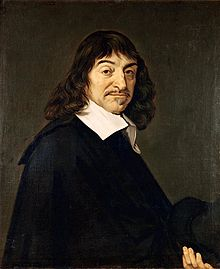
\includegraphics[height=\the\HauteurDesPhotos]{Descartes}&%
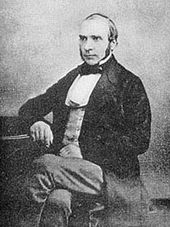
\includegraphics[height=\the\HauteurDesPhotos]{Snow}&%
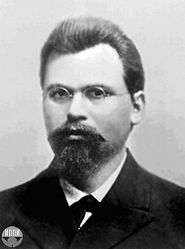
\includegraphics[height=\the\HauteurDesPhotos]{Voronoi}\\
Descartes&Snow&Voronoï%
\end{tabular}}
\medskip
\ImageADroite{%
Les diagrammes de Voronoï\index[aut]{Voronoï (Gueorgui Feodossievitch), 1868-1908, Russe} portent le nom du mathématicien russe Georgy Fedoseevich Voronoï qui a défini et étudié le cas général en dimension $n$ en 1908. Les diagrammes de Voronoï qui sont utilisés en géophysique et en météorologie pour analyser des données de distributions spatiales (comme les mesures de chutes de pluie) sont appelés polygones de Thiessen du nom du météorologiste américain Alfred H. Thiessen.\index[aut]{Thiessen (Alfred H.), 1872-1956, Américain}
Ils sont également très utiles en géométrie algorithmique, en particulier pour des problèmes de représentation ou de quantification, et sont utilisés dans le champ de la robotique pour créer un protocole pour éviter les obstacles détectés.
Pour la modélisation de phénomènes naturels, ils servent pour les études de la compétition végétale (écologie et sylviculture), pour les territoires d'animaux (zoologie) et des clans et tribus néolithiques (anthropologie et archéologie), ainsi que pour les modèles de zones urbaines (géographie). Il expliquent aussi la répartition (et la forme) des tâches du pelage des girafes et des écailles de tortues.}

\sbox{\MaBoiteAvecPhotos}{\setlength{\tabcolsep}{0pt}\scriptsize%
\begin{tabular}{c}%
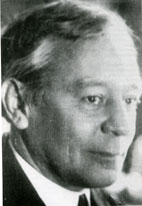
\includegraphics[height=\the\HauteurDesPhotos]{Delaunay}\\%
Delaunay%
\end{tabular}}
\medskip
\ImageAGauche{%
La triangulation de Delaunay\index[aut]{Delaunay (Boris Nikolaïevitch), 1890-1980, Russe} a été inventée par le mathématicien russe Boris Delaunay en 1934.
D'après la définition de Delaunay, le cercle circonscrit d'un triangle constitué de trois points de l'ensemble de départ est vide s'il ne contient pas d'autres sommets que les siens. Ainsi, les autres points sont autorisés sur le périmètre en lui-même mais pas à l'intérieur strict du cercle circonscrit. La condition de Delaunay affirme qu'un réseau de triangles est une triangulation de Delaunay si tous les cercles circonscrits des triangles du réseau sont vides. Ceci constitue la définition originale en deux dimensions. En remplaçant les cercles par des sphères circonscrites, il est possible d'étendre la définition à la dimension trois... mais en fait, on peut l'étendre en dimension quelconque.
\textcolorblue{Les triangulations de Delaunay maximisent le plus petit angle de l'ensemble des angles des triangles, évitant ainsi les triangles allongés.}}

\medskip
On parle souvent de la triangulation de Delaunay\index[aut]{Delaunay (Boris Nikolaïevitch), 1890-1980, Russe} comme du dual du diagramme de Voronoï\index[aut]{Voronoï (Gueorgui Feodossievitch), 1868-1908, Russe} qui lui est associé. En fait les deux sont liés de la façons suivante:
\begin{itemize}
   \item Les sommets du diagramme de Voronoï sont les centres des cercles circonscrits des triangles de la triangulation de Delaunay. Les arêtes du diagramme de Voronoï sont sur les médiatrices des arêtes de la triangulation de Delaunay;
   \item Chaque germe (ou point générateur) du diagramme de Voronoï constitue un sommet dans la triangulation de Delaunay. Ces sommets sont reliés entre eux par une arête si et seulement si les cellules sont adjacentes.
\end{itemize}
\end{histoire}



\begin{definition}[Maillage de Delaunay]\index{maillage de Delaunay-Voronoï}
On appelle \textcolorblue{maillage de Delaunay strict}, le maillage dual des diagrammes de Voronoï, construit en reliant deux points~$x^i$ et~$x^j$, si les diagrammes~$V^i$ et~$V^j$ ont un segment en commun.

Pour rendre le maillage triangulaire, il suffit de découper les polygones qui ne sont pas des triangles en triangles. Nous appelons ces maillages des \textcolorblue{maillages de Delaunay} de l'ensemble~$\mathcal{S}$.
\end{definition}
\begin{figure}[htb]
\begin{center}
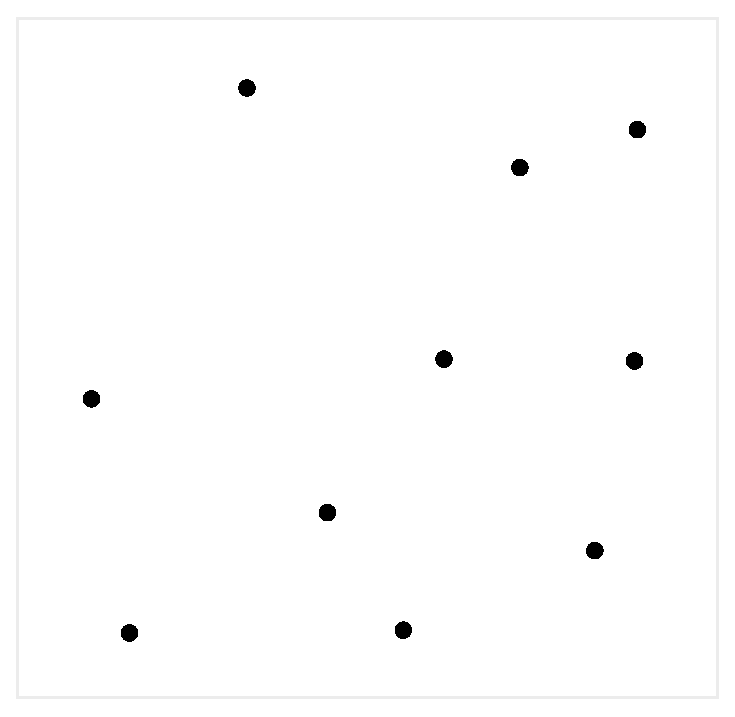
\includegraphics[height=30mm]{DV1} \hspace{1em} 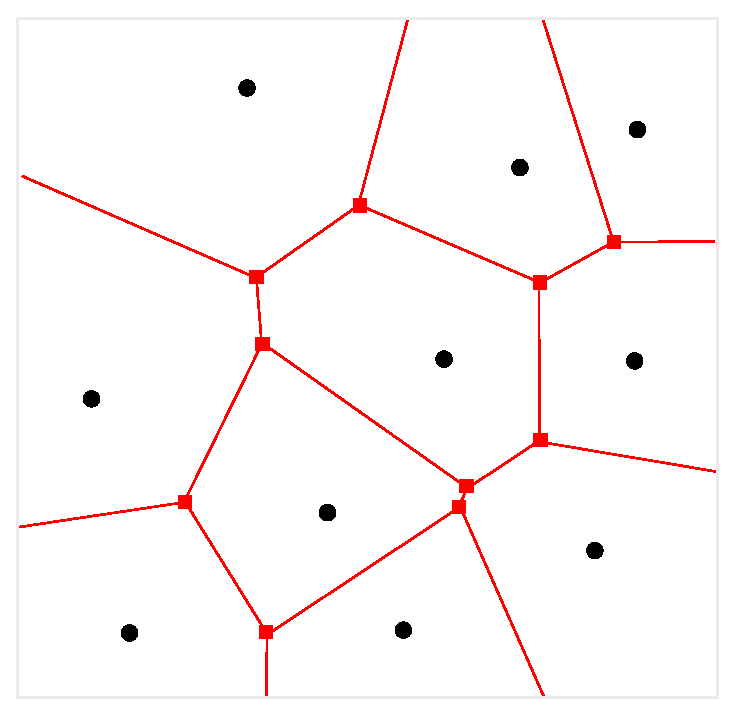
\includegraphics[height=30mm]{DV2} \hspace{1em} 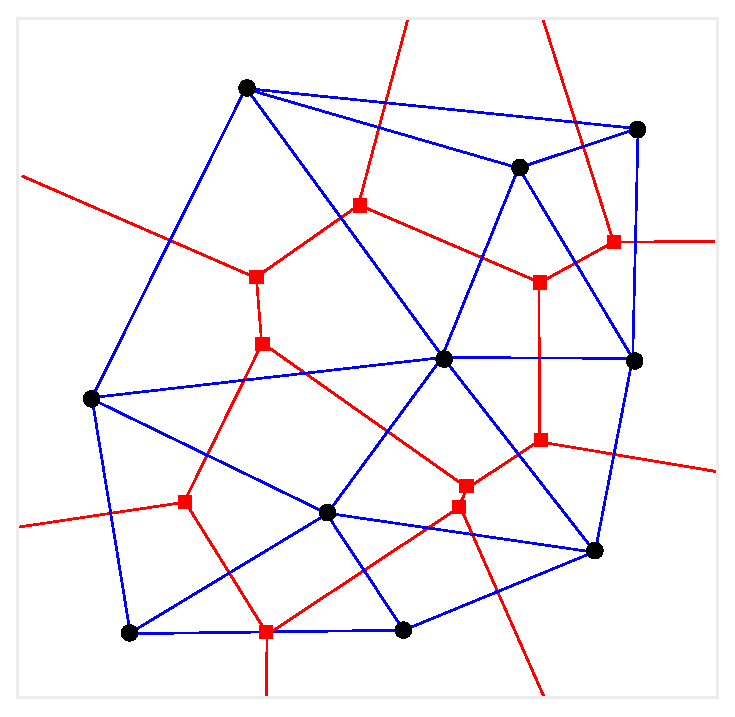
\includegraphics[height=30mm]{DV3} \hspace{1em} 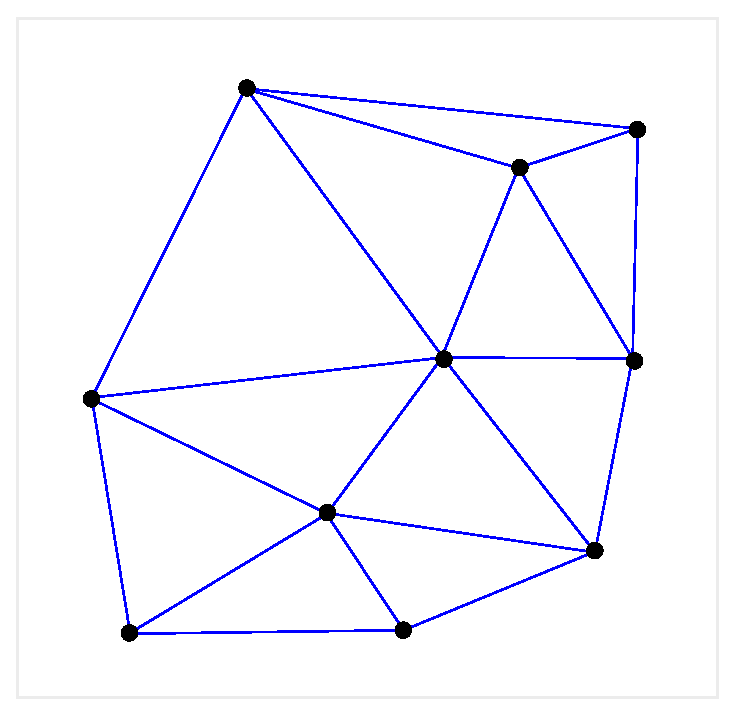
\includegraphics[height=30mm]{DV4}
\end{center}
\caption{a) points, b) ajout du diagramme de Voronoï, c) ajout de la triangulation de Delaunay et d) maillage seul}
\end{figure}

Le domaine d'un maillage de Delaunay\index[aut]{Delaunay (Boris Nikolaïevitch), 1890-1980, Russe} d'un ensemble de points~$\mathcal{S}$ est l'intérieur du convexifié~$\mathcal{C(S)}$ de l'ensemble de points~$\mathcal{S}$.

\medskip
Il existe une propriété qui permet de savoir si un maillage est un maillage de Delaunay.\index[aut]{Delaunay (Boris Nikolaïevitch), 1890-1980, Russe} C'est la propriété de la boule ouverte.
\begin{theoreme}[Propriété de la boule ouverte]\index{propriété de la boule ouverte}
Un maillage~$\mathcal{T}_{d,h}$ est un maillage de Delaunay s'il est tel que pour tout triangle~$T$ du maillage, le disque ouvert~$D(T)$ correspondant au cercle circonscrit à~$T$ ne contient
aucun sommet:
\begin{equation}
D(T) \cap \mathcal{T}_{0,h} = \emptyset
\end{equation}

Réciproquement, si le maillage~$\mathcal{T}_{d,h}$ d'un domaine convexe vérifie la propriété de la boule ouverte, alors il est de Delaunay.
\end{theoreme}
\begin{figure}[htb]
\begin{center}
 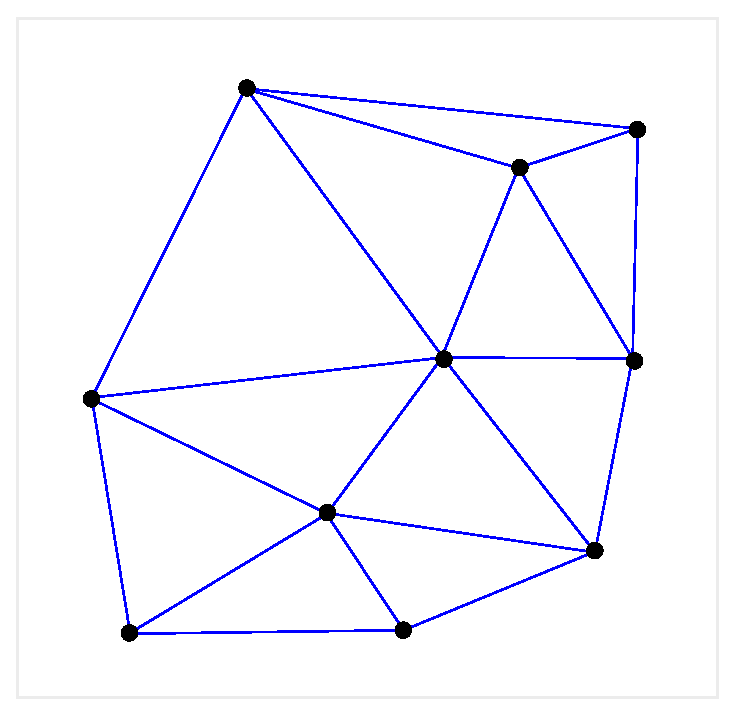
\includegraphics[height=35mm]{DV4} \hspace{1em} 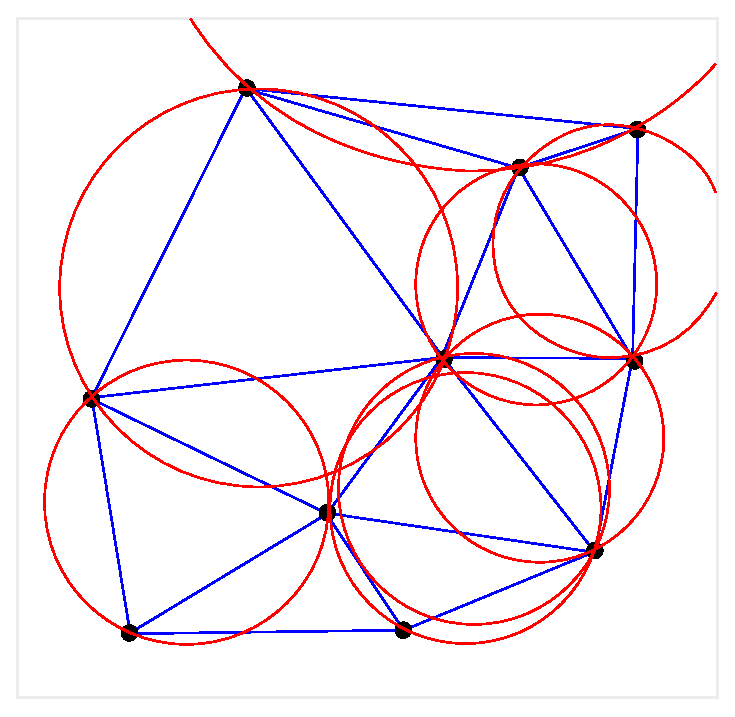
\includegraphics[height=35mm]{DV5}
\end{center}
\caption{a) Triangulation de Delaunay et b) cercles circonscrits: propriété de la boule ouverte}
\end{figure}

\medskip
La propriété de la boule ouverte peut être appliquée également au cas d'un quadrilatère convexe, puisque celui-ci peut être découpé en deux triangles adjacents. Il suffit alors de vérifier la propriété pour toutes les paires de triangles adjacents formant un quadrilatère convexe.

Si le critère de la boule ouverte n'est pas vérifié pour un quadrilatère convexe, alors on fera un échange de diagonal pour résoudre le problème.

\medskip
\subsection{Remarques}

À ce niveau, nous sommes en mesure de générer un maillage... toutefois, celui-ci n'est pas forcément exempt de problèmes:
\begin{itemize}
   \item si les seuls points disponibles sont sur la frontière, il va falloir générer des points internes au maillage. En effet, le maillage généré existe, mais peut présenter des distorsions inadmissibles en termes de calcul. Le critère le plus naturel pour distribuer les points internes est d'imposer en tout point~$x$ de~$\RR^2$, le pas de maillage~$h(x)$. En pratique, on ne dispose pas toujours de cette information et il faut la construire à partir des points disponibles, i.e. des points de la frontière. D'autre part, dans de nombreuses applications, on préfère donner le nombre de subdivisions souhaitées entre deux sommets: un peu de géométrie différentielle (longueurs d'arcs) permet de se ramener à donner une valeur à~$h(x)$;
   \item il existe des cas où le maillage généré peut ne pas respecter la frontière (par exemple pour un domaine en forme de «U» avec peu de points. Il existe une solution de forçage de la frontière par permutation d'un certain nombre de diagonales. Voir figure~\ref{Fig-Mbord};
   \item il faut traiter le cas des trous... mais ce n'est pas réellement difficile.
\end{itemize}
Comme il ne s'agit pas ici de donner un cours sur les algorithmes de maillage, nous en resterons là. Les maillages triangulaires sont plutôt bien maîtrisés. Il y a de nombreux cas à traiter pour couvrir toutes les configurations existantes, mais les bases théoriques et les réalisation pratiques existent dans tous les cas.
\begin{figure}[htb]
\begin{center}
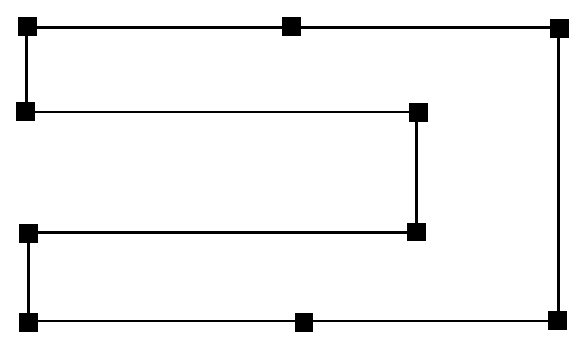
\includegraphics[height=22mm]{bord1.eps} \hspace{2em} 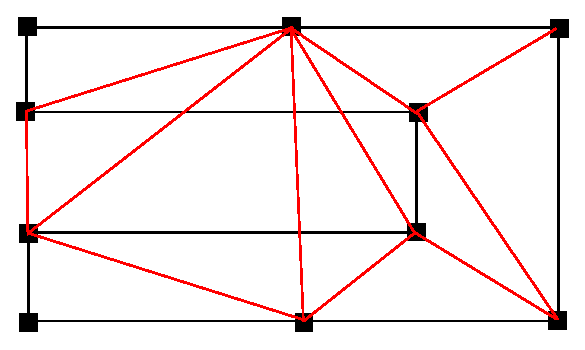
\includegraphics[height=22mm]{bord2.eps} \hspace{2em} 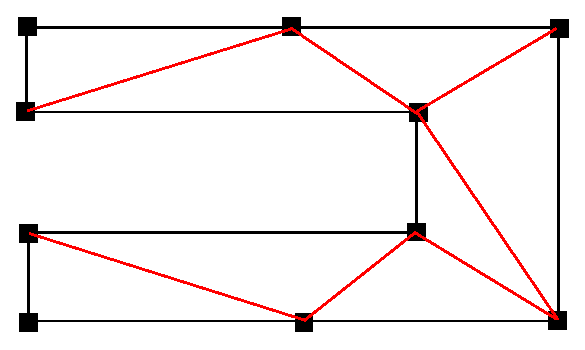
\includegraphics[height=22mm]{bord3.eps}
\end{center}
\caption{a) Points et arêtes, b) maillage de Delaunay ne respectant pas la frontière, c) maillage respectant la frontière obtenu en échangeant des diagonales}\label{Fig-Mbord}
\end{figure}

\medskip
\section{Maillage par avancement de fronts}\label{Sec-MeshFront}

Le \textcolorblue{front initial} est constitué de la frontière (ou des frontières, s'il y a des trous), i.e. des nœuds et des arêtes.
L'algorithme est très simple: pour chaque arête représentée par le segment~$[x^i,x^j]$, on crée un nouveau points~$x^{N_p+1}$ tel que le triangle formé des trois points~$x^i$, $x^j$ et~$x^{N_p+1}$ soit équilatéral.

\medskip
Évidemment il faut quelques règles supplémentaires pour que cela fonctionne bien:
\begin{itemize}
   \item on met à jour en permanence le front dès qu'un point est créé, et on ne s'arrête que lorsque toutes les arêtes du front ont été balayées;
   \item en cours de calcul, de nouveaux fronts peuvent apparaître (cela correspond à plusieurs domaines non encore maillés à l'intérieur du maillage en cours);
   \item on vérifie si des nœuds du front courant ne seraient pas candidats pour être le nouveau point~$x^{N_p+1}$ du triangle: par exemple, en s'assurant qu'un nœud existant n'appartient pas au cercle de centre le point~$x^{N_p+1}$ théorique (triangle équilatéral) et de rayon un certain paramètre fixé;
   \item lorsque plusieurs nœuds existants sont candidats, on sélectionne celui qui fournit le triangle le plus équilatéral possible;
   \item on supprime toutes les possibilités qui intersectent un front existant (pas de recouvrement d'éléments);
   \item on rejette les triangles inversés.
\end{itemize}


\medskip
\section{Maillage par transformation}\label{Sec-MeshTransfo}
% projection d'un maillage sur une sphère... voir Oudot
% voir également Hetroy

Le principe est on ne peut plus simple. Il s'agit de mettre en bijection deux domaines: d'une part le domaine à mailler compliqué~$\Omega_h$, et d'autre part un domaine de référence plus simple: rectangle, sphère...

Pour faire simple, on peut imaginer mailler une ellipse à partir du maillage d'un disque, un rectangle à partir du maillage d'un carré... on peut dire que l'\textcolorgreen{on fait du morphing sur un maillage}.
Dans la pratique, on part de la surface d'un domaine tridimensionnel complexe. On transforme cette surface en une surface plane par une certaine transformation. On maille cette nouvelle surface dans le plan. Puis on effectue la transformation inverse afin de disposer d'un maillage de la surface dans~$\RR^3$.

\ifVersionDuDocEstVincent\medskip\else\newpage\fi
\begin{wrapfigure}{l}{60mm}
\begin{center}
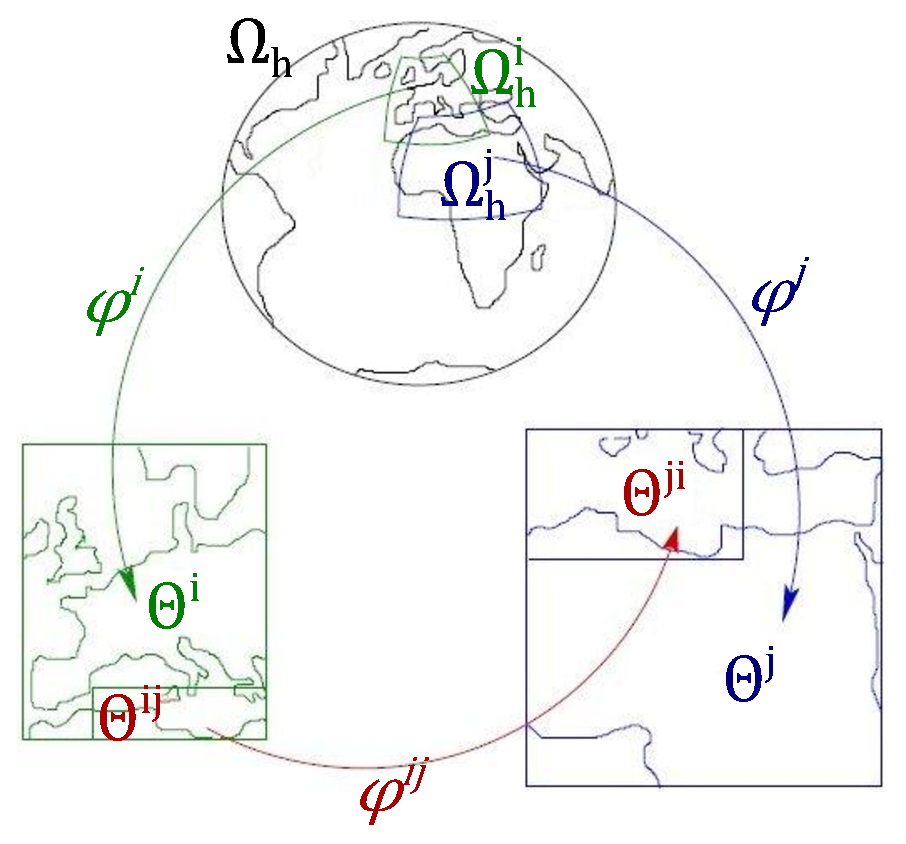
\includegraphics[width=60mm]{atlas.eps}
\end{center}
\caption{Domaines et transformations}\label{Fig-atlas}
\end{wrapfigure}
Considérons que nous souhaitions mailler notre domaine~$\Omega_h$ qui est une surface dans~$\RR^2$ ou~$\RR^3$.
On appelle \textcolorblue{transformation}~$\varphi$, un homéomorphisme transformant~$\Omega_h$ en un autre domaine (plus simple par exemple, ou au moins plan si la surface de~$\Omega_h$ est dans~$\RR^3$) noté~$\Theta$.
Comme nous utilisons des homéomorphismes, les transformations inverses existent et sont continues. Nous sommes donc en mesure de repasser de~$\Theta$ à~$\Omega_h$.

Dans le cas général, illustré à la figure~\ref{Fig-atlas}, ce domaine~$\Omega_h$ peut lui-même être déjà décomposé en un certain nombre de sous-domaines~$\Omega_h^i$ avec recouvrement partiel des sous-domaines \textcolorgris{(les~$\Omega_h^i$ sont des ouverts de la variété~$\Omega_h$)}.
On appelle \textcolorblue{transformations}~$\varphi^i$, les homéomorphismes transformant~$\Omega_h^i$ en les sous-domaines~$\Theta^i$ (avec recouvrements partiels) constituant~$\Theta$.
On appelle \textcolorblue{fonctions de transition}~$\varphi^{ij}$ les transformations permettant de passer du sous-domaine~$\Theta^{ij}$ de~$\Theta^i$ correspondant à la zone de recouvrement dans~$\Theta^i$ avec~$\Theta^j$ au sous-domaine~$\Theta^{ji}$ de~$\Theta^j$ correspondant à la zone de recouvrement dans~$\Theta^j$ avec~$\Theta^i$. Cela permet de s'assurer de la bonne transition entre les \textcolorblue{cartes} locales~$\Theta^{i}$ \textcolorgris{(les~$\Theta^i$ forment un atlas de cartes)}.

\medskip
La transformation considérée peut conserver une ou plusieurs des propriétés suivantes:
\begin{itemize}
   \item les angles: transformation conforme;
   \item les aires: transformation authalique;
   \item les longueurs: transformation isométrique.
\end{itemize}

\medskip
Un cas «simple» est celui où~$\Omega_h$ est une \textcolorblue{surface de genre zéro sans bord} (une telle surface correspond à la surface d'un volume sans trou, c'est donc quelque chose de très général).
Une surface de genre zéro sans bord est homéomorphe à la sphère unité~$S^2$ et l'on peut donc trouver un homéomorphisme~$\varphi$, qui peut être compliqué, entre~$\Omega_h$ et la sphère, i.e. on est dans la cas précédent où l'on passe directement de~$\Omega_h$ à~$S^2$ par un unique homéomorphisme~$\varphi$. Il ne reste plus ensuite qu'à mailler la sphère, puis à envoyer tous les sommets du maillage sur~$\Omega_h$ par~$\varphi^{-1}$, tout en conservant la même connectivité. Il faut toutefois veiller à mailler~$S^2$ assez finement pour s'assurer que le maillage de~$\Omega_h$ ne s'auto-intersecte pas. Ainsi, la densité locale des sommets du maillage de~$S^2$ doit dépendre de~$\Omega_h$, et donc de~$\varphi$.

Le maillage de la sphère n'est pas si simple qu'on le pense.
On peut là encore appliquer la même technique: définir un homéomorphisme entre la demi-sphère et le disque, mailler le disque. Le maillage de la sphère, obtenu par symétrie de la demi-sphère doit alors «se recoller», du moment que le maillage du bord du cercle est conforme et laissé conforme par l'homéomorphisme. Si l'on procède au maillage du cercle par la méthode de Delaunay\index[aut]{Delaunay (Boris Nikolaïevitch), 1890-1980, Russe} telle que décrite en partant du contour du cercle, on est alors assuré que le maillage du contour sera conforme.

Dans les deux cas, passage du cercle à la demi-sphère et passage de la sphère à~$\Omega_h$, on pourra remarquer que la densité du maillage n'est généralement pas la même. Il s'agit du \textcolorblue{phénomène d'étirement}. Si l'on souhaite que la surface finale~$\Omega_h$ ait une densité de maillage fixée, il faut savoir comment~$\varphi^{-1}$ modifie cette densité pour pouvoir mailler~$S^2$ en conséquence... idem pour le cercle. Cela n'est pas simple, surtout si~$\Omega_h$ est compliqué.

\medskip\ifVersionDuDocEstVincent\else\newpage\fi
\section{Remarques sur le maillage quadrangulaire et hexaédrique}\label{Sec-MeshQuad}

\begin{wrapfigure}{r}{45mm}
\begin{center}
\includegraphics[width=45mm]{SphereLW.jpg}
\end{center}
\caption{Maillage en quadrangles d'aires égales}\label{Fig-sphereLW}
\end{wrapfigure}
Même en 2D, il est plus difficile de générer un maillage quadrangulaire que triangulaire.
Une raison fondamentale est que tout polygone ne peut être décomposé en un ensemble de quadrangles: il peut être nécessaire d'ajouter des sommets sur le bord. Et \textcolorgreen{en pratique, il est nécessaire et suffisant d'avoir un nombre pair d'arêtes sur le bord géométrique.}

En 3D, on ne peut pas mailler tout volume dont le bord est maillé par une surface quadrangulaire.
Disposer d'un nombre pair de quadrangles sur le bord n'est qu'une condition nécessaire.
\textcolorgreen{Une condition suffisante est d'avoir un nombre pair de quadrangles maillant une surface topologiquement équivalente à une sphère. Dans ce cas, le volume délimité par la surface en question admet un maillage hexaédrique.}

Le \textcolorblue{maillage d'une sphère en quadrangles de même aire} est un problème difficile qui ressort du problème de Tammes, ou problème des dictateurs. Une solution a été donnée par Lemaire\index[aut]{Lemaire (Christophe), ?-, Français} et Weill\index[aut]{Weill (Jean-Christophe), ?-, Français} en 2000~\cite{bib-LemW}. Un maillage obtenu est donné à la figure~\ref{Fig-sphereLW}. Un tel maillage comporte $24n^2$ éléments par construction: la sphère est «découpée» par son cube inscrit et chacun des six morceaux obtenus est divisé en quatre par symétrie. Toutefois, il faut noter que les quadrangles considérés ne sont pas plans, ce sont des morceaux de sphères. Pour l'instant il n'y a pas de solution «parfaitement satisfaisante» avec des quadrangles plans, dans un sens qui reste à définir... puisque l'invariant d'Euler-Poincaré\index[aut]{Euler (Leonhard Paul), 1707-1783, Suisse}\index[aut]{Poincaré (Henri), 1854-1912, Français} implique par exemple qu'il n'y a pas de polygonalisation de la sphère (qui est de caractéristique d'Euler-Poincaré de 2) avec uniquement des rectangles (ou des hexagones d'ailleurs). Au passage, rappelons que les triangles permettent eux une polygonalisation d'une surface, quelque soit sa caractéristique, d'où leur succès... mais attention à réaliser une maillage «pas trop trivial» afin d'éviter le cas de triangles trop distordus venant se connecter sur un même sommet et conduisant à des singularités en terme de calcul numérique (et pour cela, utilisons donc la triangulation de Delaunay-Voronoï).

\medskip
Aucune méthode n'est apte à traiter tous les cas possibles concernant le maillage avec des quadrangles ou des hexaèdres. Néanmoins de nombreux algorithmes sont disponibles:
\begin{itemize}
   \item Les \textcolorblue{maillages structurés} (obtention de la répétition régulière de motifs identiques) fonctionnent bien mais ne sont pas adaptés à toutes les géométries.
   \item On peut \textcolorblue{subdiviser} le domaine en plusieurs parties pour appliquer sur chacune d'elles un maillage structuré ou un maillage obtenu par déformation d'un maillage structuré.
   \item On peut définir deux faces topologiquement équivalentes du modèles comme les surfaces source et cible et découper les surfaces de liaisons entre la source et la cible pour créer un \textcolorblue{maillage structuré dans une direction}.
   \item On peut raisonner comme en CAO en générant des maillages par extrusion ou par révolution.
   \item Le \textcolorblue{paving} est une variante de l'avancée de front. On essaye de faire un maillage de type structuré en reportant un front «parallèle» au front existant, avec le même nombre de nœuds. Il sera nécessaire d'avoir des distorsions  à certains endroits et autour des trous, il faudra faire des coutures.
   \item Le \textcolorblue{Q-morph} se propose de de transformer un maillage triangulaire en maillage quadrangulaire par avancée de front. Cela ne fonctionne pas en 3D.
   \item Les \textcolorblue{méthodes basées sur une grille} considèrent la surface ou le volume découpé(e) en carrés ou cubes selon une grille prédéfinie. Il suffit alors d'adapter les éléments situés au bord du domaine: ceux-ci seront de moins bonne qualité et parfois même pas totalement conformes au bord théorique.
\end{itemize}
Le maillage quadrangulaire et surtout hexaédrique reste un domaine de recherche actif.
